\section{Embedded Computer System}
An \concept{embedded computer system} is a special purpose computer system where the computer is \emph{embedded} in the device it controls.
These computers are much smaller than conventional server, desktop, and laptop computers, but are by far more numerous.
A regular household contains embedded systems in devices like microwave ovens, dishwashers, and alarm systems.
In a car you find embedded computers which are controlling the breaks of the car, the automatic windows, and navigation and entertainment systems.

In recent years, a trend of devices called wearables are emerging, which also has an embedded computer at its core.
The internet is growing, and according to Gartner \cite{web:gartner} the number of connected devices will increase form $\sim$5 billion in 2015 to $\sim$25 billion by 2020.
A vast majority of this increase is due to the embedded computer systems known as the \gls{iot} \cite{Valhouli2010}.

\subsection{Abstraction Level}
In most computer systems, the hardware interaction and resource management is abstracted away with an \gls{os}.
This abstraction layer makes it possible for the programmers of these systems to write portable programs built with higher level languages.
The added complexities of using a high level language are small enough compared to the added productivity and convenience for the programmer.
Some embedded system are also based on an \gls{os}, projects like Raspberry PI\footnote{\url{https://www.raspberrypi.org/}} and Tessel\footnote{\url{https://tessel.io/}} employs reduced Linux versions to run Python and JavaScript respectively.

In some embedded system, these complexities which leads to lower performance and higher memory usage, makes it hard to benefit from an \gls{os}.
With the absence of an \gls{os}, applications for embedded system are usually written in a lower level languages.
These languages must provide the low level control which is needed by the programmer to interact directly with the hardware.
A well known project running without an \gls{os} is the electronic prototyping platform Arduino\footnote{\url{http://www.arduino.cc/}}.
The EFM32 {\emlib} library used in this thesis is also a platform for {\C} programming without an \gls{os}.

In this thesis we use the words \emph{embedded} and \emph{bare-metal} interchangeably, to refer to execution of code directly on the hardware, without the abstraction of an \gls{os}.
This is the only execution mode that we have targeted in this project.

\subsection{Programming Model}

A common programming model used in embedded systems is the \emph{Event-driven} programming model.
In this model, the program is controlled by events which in turn triggers actions to be executed.
Within an embedded system, these events are hardware interrupts, and the actions are handler functions dispatched by the runtime system.
A typical example of this event-action pair is the interrupts that are issued by pressing a button and the action turning on a LED.

Other events that triggers interrupt handlers to be executed in an embedded system is timers, sensors with available data, and communication peripherals ready to receive or send data.
This programming model is successful in these systems because the peripherals controlled by the \gls{mcu} usually requires time to perform its operation.
The asynchronous nature of the model lets the \gls{cpu} avoid the busy-waits that are implied when using a more synchronous model.

\subsection{Programming Language}

Lower-level languages have usually been the preferred ones for programming of embedded systems.
Traditionally, a large portion of code bases consists of {\C}, \lang{Assembly}, and {\Cpp}.
As seen in \autoref{fig:vdc:langs} according to VDC Research \cite{web:vdc} survey language used in embedded systems, the usage of C and assembly are on the way down in favor for higher level languages like C++, Java, and C\#.

\begin{figure}[H]
  \begin{center}
    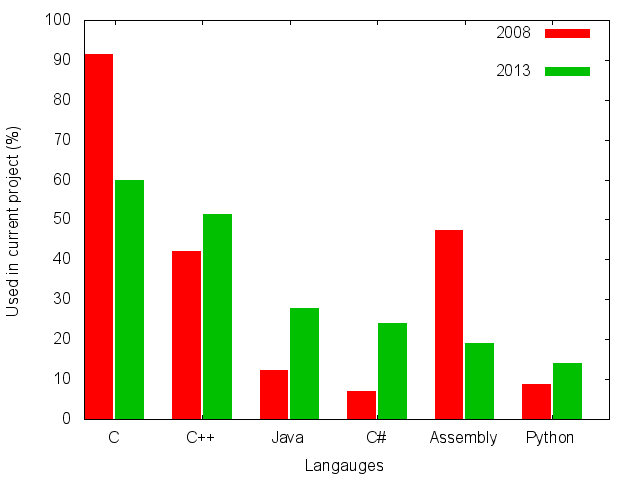
\includegraphics[scale=0.5]{figures/plots/langs.png}
  \end{center}
  \caption{Survey of language used on current embedded system project by VDC Research}
  \label{fig:vdc:langs}
\end{figure}

The runtime system for \emph{managed} languages like {\Java}, \lang{Python}, and \lang{C\#}, features automatic memory management.
This memory management lets the language ensure memory safety, but incurs a runtime cost and can make performance analysis non-deterministic.
When these languages are used for bare-metal programming the memory management is usually altered \cite{PetitBianco} \cite{Pizlo} \footnote{\url{http://en.wikipedia.org/wiki/.NET_Micro_Framework}}.

\subsection{Benefits of the Rust language}
The {\rust} programming language implements a novel approach to \emph{memory management} based on region based memory management from \lang{Cyclone} \cite{Grossman2002,Swamy2006}, among others.
This kind of memory management substitutes the runtime checks, performed by an automatic memory manager, to a static analysis performed by the compiler.
This lets the {\rust} language ensure memory safety without the runtime cost of automatic memory management.

One of the design goals for {\rust} is to provide \emph{Zero-Cost Abstractions}.
One implication of this goal is that abstractions in {\rust} should not have worse performance than the same, less abstracted, code in other low-level languages.
This design goal makes the language a good fit for embedded systems as costly abstractions could have rendered parts of the language useless.

{\rust} has a distinction between \emph{safe} and \emph{unsafe} code.
For this, {\rust} provides a concept of {\unsafe} sections where the compiler relies on the programmer to ensure that the safe invariants are maintained.
This section can be used when building abstractions in {\rust}, as the compilers rules for ensuring safety can sometimes become too strict.
Containing these sections in {\unsafe} sections makes it easier for the programmer to reason about the safety of the code.

The {\rust} language is developed by the Mozilla Foundation.
With this foundation comes a range of \emph{Open Source} projects and a vibrant community.
This makes the community around {\rust} an open and inviting space to share knowledge and code.
The {\rust} language and compiler is developed in the open on the GitHub\footnote{\url{https://github.com/}} code collaboration platform, which makes for a low entry cost both in learning from the project and contributing to it.
Throughout the work for this thesis we have both had a huge benefit of the openness of the development, and had the chance to contribute with code back to project.

One particularly good tool for sharing and building {\rust} projects is the {\cargo} package manager.
This tool makes sharing and reusing libraries of code very easy.

\subsection{The RustyGecko Platform}

In this thesis we develop and evaluate the \textbf{RustyGecko} platform, a bare-metal platform for {\rust} on the EFM32 series of \glspl{mcu}.
The platform is described by \autoref{fig:rustygecko:all}.
The blue colored sections describe the {\rust} modules that were developed/fitted for the platform, and the brown/yellow sections show the base {\C} libraries that the platform utilizes.
The orange section denotes the build system.

\begin{figure}[H]
  \begin{center}
    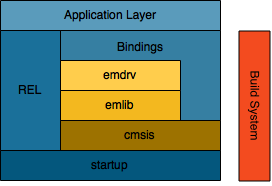
\includegraphics{figures/RustyGecko-all.png}
  \end{center}
  \caption{The contents of the RustyGecko platform}
  \label{fig:rustygecko:all}
\end{figure}

\autoref{fig:rustygecko:all} is described in a bottom-up perspective throughout \autoref{chap:impl}.
The \lib{startup} module deals with the minimal requirements for booting a {\rust} application on the \gls{mcu} and is described in \autoref{sec:impl:booting}.
In \autoref{sec:rel} we define \gls{rel}, the subset of the {\rust} standard library which is applicable for embedded systems.

In the center part of the figure we find the peripheral libraries for controlling both the \gls{mcu} and its connected devices, these are used in {\rust} through language bindings.
The details of these libraries and implementations are given in \autoref{sub:interfacing_with_emlib}.
In \autoref{sec:build_system} we take a detour and look at the building system used to support development on the {\rg} platform.
Lastly, we consider some high-level libraries and applications that we place in the Application Layer platform.

The {\rg} platform as a whole aims to bring the safety and high level abstractions of {\rust} to embedded computer systems.